%\documentclass[12pt,reqno,oneside]{puctesis}         % For dvips
\documentclass[12pt,reqno,oneside,pdftex]{formato-puc/puctesis} % For pdflatex
%\documentclass[10pt,reqno,twoside]{puctesis}
%\draft
%\doublespacing
%\usepackage{verbatim}
%\usepackage{setspace}
\usepackage{graphicx}
\usepackage{amsmath}
\usepackage{amsfonts}
\usepackage{amssymb}
\usepackage[spanish]{algorithm2e}
\usepackage{fancybox}
\usepackage{float}
\usepackage{times}

\usepackage{color}
\usepackage{fancyvrb}
\newcommand{\VerbBar}{|}
\newcommand{\VERB}{\Verb[commandchars=\\\{\}]}
\DefineVerbatimEnvironment{Highlighting}{Verbatim}{commandchars=\\\{\}}
\usepackage{framed}
\definecolor{shadecolor}{RGB}{248,248,248}
\newenvironment{Shaded}{\begin{snugshade}}{\end{snugshade}}
\newcommand{\AlertTok}[1]{\textcolor[rgb]{0.94,0.16,0.16}{#1}}
\newcommand{\AnnotationTok}[1]{\textcolor[rgb]{0.56,0.35,0.01}{\textbf{\textit{#1}}}}
\newcommand{\AttributeTok}[1]{\textcolor[rgb]{0.77,0.63,0.00}{#1}}
\newcommand{\BaseNTok}[1]{\textcolor[rgb]{0.00,0.00,0.81}{#1}}
\newcommand{\BuiltInTok}[1]{#1}
\newcommand{\CharTok}[1]{\textcolor[rgb]{0.31,0.60,0.02}{#1}}
\newcommand{\CommentTok}[1]{\textcolor[rgb]{0.56,0.35,0.01}{\textit{#1}}}
\newcommand{\CommentVarTok}[1]{\textcolor[rgb]{0.56,0.35,0.01}{\textbf{\textit{#1}}}}
\newcommand{\ConstantTok}[1]{\textcolor[rgb]{0.00,0.00,0.00}{#1}}
\newcommand{\ControlFlowTok}[1]{\textcolor[rgb]{0.13,0.29,0.53}{\textbf{#1}}}
\newcommand{\DataTypeTok}[1]{\textcolor[rgb]{0.13,0.29,0.53}{#1}}
\newcommand{\DecValTok}[1]{\textcolor[rgb]{0.00,0.00,0.81}{#1}}
\newcommand{\DocumentationTok}[1]{\textcolor[rgb]{0.56,0.35,0.01}{\textbf{\textit{#1}}}}
\newcommand{\ErrorTok}[1]{\textcolor[rgb]{0.64,0.00,0.00}{\textbf{#1}}}
\newcommand{\ExtensionTok}[1]{#1}
\newcommand{\FloatTok}[1]{\textcolor[rgb]{0.00,0.00,0.81}{#1}}
\newcommand{\FunctionTok}[1]{\textcolor[rgb]{0.00,0.00,0.00}{#1}}
\newcommand{\ImportTok}[1]{#1}
\newcommand{\InformationTok}[1]{\textcolor[rgb]{0.56,0.35,0.01}{\textbf{\textit{#1}}}}
\newcommand{\KeywordTok}[1]{\textcolor[rgb]{0.13,0.29,0.53}{\textbf{#1}}}
\newcommand{\NormalTok}[1]{#1}
\newcommand{\OperatorTok}[1]{\textcolor[rgb]{0.81,0.36,0.00}{\textbf{#1}}}
\newcommand{\OtherTok}[1]{\textcolor[rgb]{0.56,0.35,0.01}{#1}}
\newcommand{\PreprocessorTok}[1]{\textcolor[rgb]{0.56,0.35,0.01}{\textit{#1}}}
\newcommand{\RegionMarkerTok}[1]{#1}
\newcommand{\SpecialCharTok}[1]{\textcolor[rgb]{0.00,0.00,0.00}{#1}}
\newcommand{\SpecialStringTok}[1]{\textcolor[rgb]{0.31,0.60,0.02}{#1}}
\newcommand{\StringTok}[1]{\textcolor[rgb]{0.31,0.60,0.02}{#1}}
\newcommand{\VariableTok}[1]{\textcolor[rgb]{0.00,0.00,0.00}{#1}}
\newcommand{\VerbatimStringTok}[1]{\textcolor[rgb]{0.31,0.60,0.02}{#1}}
\newcommand{\WarningTok}[1]{\textcolor[rgb]{0.56,0.35,0.01}{\textbf{\textit{#1}}}}

% --- START: Babel ---
% Esta seccion es necesaria para quienes desean usar Babel y acentos
% en castellano en vez de acentos LaTeX tradicionales, e.j. \'a, \'e, etc.
% Como Babel tiene un manejo distinto al normal para definir los nombres
% de las partes del documento no basta con usar \renewcommand{\...name}
% sino que es necesario usar tambi\'en \addto\captionspanish.
% MTT 2011.11.30
\usepackage[spanish]{babel}    % Estos paquetes alteran las definiciones
\usepackage[utf8]{inputenc}
%\usepackage[latin1]{inputenc}  % estandar de los titulos y requieren 
                               % redefiniciones adicionales
\addto\captionsspanish{%
  \renewcommand{\contentsname}{INDICE GENERAL}%
}
\addto\captionsspanish{
 \renewcommand{\listfigurename}{INDICE DE FIGURAS}%
}
\addto\captionsspanish{
 \renewcommand{\listtablename}{INDICE DE TABLAS}%
}
\addto\captionsspanish{
 \renewcommand{\chaptername}{}%CAPITULO}
}
\addto\captionsspanish{
 \renewcommand{\figurename}{Figura}%
}
\addto\captionsspanish{
 \renewcommand{\tablename}{Tabla}%
}
\addto\captionsspanish{
 \renewcommand{\refname}{BIBLIOGRAFIA}%
}
\addto\captionsspanish{
 \renewcommand{\bibname}{}%
}
\addto\captionsspanish{
 \renewcommand{\BOthers}[1]{et al.\hbox{}}%
}
% --- END: Babel ---

           %%%%%%%%%%%%%%%%%%%%%%%%%%%%%%%%%%%%%%%%%%%%%%%%%%%%
           %   Preambulo                                      %
           %------------------------------------------------- %
           %        \newcommand\...{...}                      %
           %        \newtheorem{}{}[]                         %
           %        \numberwithin{}{}                         %
           %%%%%%%%%%%%%%%%%%%%%%%%%%%%%%%%%%%%%%%%%%%%%%%%%%%%


%--------- NUEVOS ENTORNOS ---------
\newtheorem{definicion}{\bf Definici\'on}[chapter]
\newtheorem{propiedad}{Propiedad}[chapter]
\newtheorem{afirmacion}{Afirmaci\'on}[chapter]
\newtheorem{lema}{\bf Lema}[chapter]
\newtheorem{proposicion}{Proposici\'on}[chapter]
\newtheorem{teorema}{\noindent \bf Teorema}[chapter]
\newtheorem{corolario}{\bf Corolario}[chapter]
\newtheorem{pf}{Demostraci\'on}[chapter]
\newtheorem{ejemplo}{\bf Ejemplo}[chapter]
\newtheorem{comentario}{Comentario}[chapter]

%--------- COLOQUE ENTORNOS/DEFINICIONES ADICIONALES AQUI ---------

\newcommand\opgrad{\operatorname{grad}}        
% ...


%----------------------------------------------------------------------%
\begin{document}

           %%%%%%%%%%%%%%%%%%%%%%%%%%%%%%%%%%%%%%%%%%%%%%%%%%%%
           %                                                  %
           %  INICIALIZACIONES : PORTADA                      %
           %                                                  %
           %%%%%%%%%%%%%%%%%%%%%%%%%%%%%%%%%%%%%%%%%%%%%%%%%%%%
%\draft                        %a?ade nota al pie con fecha del borrador
\mdate{April 17, 2007}         %fecha de modificacion del manuscrito
\version{1}                    %numero de version del manuscrito


\title{Fórmula de la media y la serie geométrica, tesis de ejemplo}
\author{PACHÁ}

\facultyto    {Departamento de Estadística}
\faculty      {Facultad de Derecho}
\address{Facultad de Derecho\\
         Pontificia Universidad Cat\'olica de Chile\\ 
         Vicu\~na Mackenna 4860\\
         Santiago, Chile\\
         {\it Tel.\/} : 56 (2) 354-2000}
\degree       {Magíster en Estadística} 
\advisor      {Nombre del profesor guía}
\subject      {Estimación de parámetros}
\date         {Diciembre 2019}
\copyrightname{SIMPLEMENTE PACHÁ}
\copyrightyear{MMXIX}
\dedication   {A mi familia, amigos y personas valiosas de la universidad}

           %%%%%%%%%%%%%%%%%%%%%%%%%%%%%%%%%%%%%%%%%%%%%%%%%%%%
           %   PRELIMINARIDADES                               %
           %--------------------------------------------------%
           %      pags. i & ii: segunda pagina                %
           %      pags. iii: dedicatoria                      %
           %%%%%%%%%%%%%%%%%%%%%%%%%%%%%%%%%%%%%%%%%%%%%%%%%%%%

\PageNumbersFootCentered       % numeros de pagina centrados en el pie															
\pagenumbering{roman}
\maketitle


           %%%%%%%%%%%%%%%%%%%%%%%%%%%%%%%%%%%%%%%%%%%%%%%%%%%%
           %   PAGINAS EXTRA                                  %
           %--------------------------------------------------%
           %      pags. --: not used                          %
           %%%%%%%%%%%%%%%%%%%%%%%%%%%%%%%%%%%%%%%%%%%%%%%%%%%%

%\newpage
%\thispagestyle{empty}

%----------------------------------------------------------------------%

           %%%%%%%%%%%%%%%%%%%%%%%%%%%%%%%%%%%%%%%%%%%%%%%%%%%%
           %      pags. iv: AGRADECIMIENTOS                   %
           %%%%%%%%%%%%%%%%%%%%%%%%%%%%%%%%%%%%%%%%%%%%%%%%%%%%

\chapter*{AGRADECIMIENTOS}
Esta plantilla de R Markdown se base en la plantilla Latex hecha por
Miguel Torres Torriti. Los agradecimientos se editan directamente en formato-puc/base.tex.
\par
%\bigskip

%................................

\cleardoublepage % En la impresion en doble cara, este comando hace que
                 % la siguiente pagina sea una pagina derecha
                 % (es decir, un pagina con numero impar con respecto
                 % a la cuenta absoluta), produciendo una pagina en blanco
                 % si es necesario.  Agregado por MTT 20.AUG.2002

%----------------------------------------------------------------------%

           %%%%%%%%%%%%%%%%%%%%%%%%%%%%%%%%%%%%%%%%%%%%%%%%%%%%
           %      pags. v & up ---                            %
           %            Indice General                        %
           %            Lista de Figuras                      %
           %            Lista de Tablas                       %
           %%%%%%%%%%%%%%%%%%%%%%%%%%%%%%%%%%%%%%%%%%%%%%%%%%%%

\tableofcontents
\listoffigures          
\listoftables           
\cleardoublepage % En la impresion en doble cara, este comando hace que
                 % la siguiente pagina sea una pagina derecha
                 % (es decir, un pagina con numero impar con respecto
                 % a la cuenta absoluta), produciendo una pagina en blanco
                 % si es necesario.  Agregado por MTT 20.AUG.2002

%----------------------------------------------------------------------%

           %%%%%%%%%%%%%%%%%%%%%%%%%%%%%%%%%%%%%%%%%%%%%%%%%%%%
           %      pags. x & xi: RESUMEN - ABSTRACT
           %%%%%%%%%%%%%%%%%%%%%%%%%%%%%%%%%%%%%%%%%%%%%%%%%%%%


\chapter*{RESUMEN}

El resumen del trabajo se edita directamente en formato-puc/base.tex.

\cleardoublepage % In double-sided printing style makes the next page 
                 % a right-hand page, (i.e. a truly odd-numbered page 
                 % with respect to absolut counting), producing a blank
                 % page if necessary. Added by MTT 20.AUG.2002 

%======================================================================%

           %%%%%%%%%%%%%%%%%%%%%%%%%%%%%%%%%%%%%%%%%%%%%%%%%%%%
           %   TEXTO DE LA TESIS
           %%%%%%%%%%%%%%%%%%%%%%%%%%%%%%%%%%%%%%%%%%%%%%%%%%%%

\NoChapterPageNumber           % elimina encabezado - pie de pagina de la
                               % primera pagina de cada capitulo
\pagenumbering{arabic}

           %%%%%%%%%%%%%%%%%%%%%%%%%%%%%%%%%%%%%%%%%%%%%%%%%%%%
           %   TEXTO DE LA TESIS
           %%%%%%%%%%%%%%%%%%%%%%%%%%%%%%%%%%%%%%%%%%%%%%%%%%%%

\chapter{NOMBRE DEL CAPITULO 1}

\hypertarget{seccion-1}{%
\section{SECCION 1}\label{seccion-1}}

Texto de ejemplo: Sed ut perspiciatis unde omnis iste natus error sit
voluptatem accusantium doloremque laudantium, totam rem aperiam, eaque
ipsa quae ab illo inventore veritatis et quasi architecto beatae vitae
dicta sunt explicabo. Nemo enim ipsam voluptatem quia voluptas sit
aspernatur aut odit aut fugit, sed quia consequuntur magni dolores eos
qui ratione voluptatem sequi nesciunt. Neque porro quisquam est, qui
dolorem ipsum quia dolor sit amet, consectetur, adipisci velit, sed quia
non numquam eius modi tempora incidunt ut labore et dolore magnam
aliquam quaerat voluptatem. Ut enim ad minima veniam, quis nostrum
exercitationem ullam corporis suscipit laboriosam, nisi ut aliquid ex ea
commodi consequatur? Quis autem vel eum iure reprehenderit qui in ea
voluptate velit esse quam nihil molestiae consequatur, vel illum qui
dolorem eum fugiat quo voluptas nulla pariatur?

\hypertarget{sub-seccion-1}{%
\subsection{SUB-SECCION 1}\label{sub-seccion-1}}

Texto de ejemplo: At vero eos et accusamus et iusto odio dignissimos
ducimus qui blanditiis praesentium voluptatum deleniti atque corrupti
quos dolores et quas molestias excepturi sint occaecati cupiditate non
provident, similique sunt in culpa qui officia deserunt mollitia animi,
id est laborum et dolorum fuga. Et harum quidem rerum facilis est et
expedita distinctio. Nam libero tempore, cum soluta nobis est eligendi
optio cumque nihil impedit quo minus id quod maxime placeat facere
possimus, omnis voluptas assumenda est, omnis dolor repellendus.
Temporibus autem quibusdam et aut officiis debitis aut rerum
necessitatibus saepe eveniet ut et voluptates repudiandae sint et
molestiae non recusandae. Itaque earum rerum hic tenetur a sapiente
delectus, ut aut reiciendis voluptatibus maiores alias consequatur aut
perferendis doloribus asperiores repellat.

\hypertarget{seccion-2}{%
\section{SECCION 2}\label{seccion-2}}

Por completitud incluyo una cita en Bibtex: Bock, Velleman, and De Veaux
(2010) contiene la ecuación de la media ponderada.

También podríamos decir ``la definición de media ponderada es \ldots{}
(Bock, Velleman, and De Veaux 2010)''.

\chapter{NOMBRE DEL CAPITULO 2}

\hypertarget{seccion-1-algunas-ecuaciones}{%
\section{SECCION 1: ALGUNAS
ECUACIONES}\label{seccion-1-algunas-ecuaciones}}

\hypertarget{serie-geomuxe9trica}{%
\subsection{Serie geométrica}\label{serie-geomuxe9trica}}

Sea \(r\in (0,1)\) se tiene que la suma de exponentes consecutivos de
\(r^i\) converge, es decir \begin{equation}
\sum_{i=0}^{\infty} r^i = \frac{1}{1-r}
\end{equation} notamos que \(r\) puede crecer de manera tal que \[
\lim_{r\to \infty} \frac{1}{1-r} = 0
\] o escrito de otra manera \[
\sum_{i=0}^{\infty} r^i = \frac{1}{1-r} \stackrel{r\to \infty}{\longrightarrow} 0
\]

\hypertarget{distribuciuxf3n-normal}{%
\subsection{Distribución Normal}\label{distribuciuxf3n-normal}}

\begin{equation}
\mathcal{N}(\mu,\sigma^2) = \int\limits_{-\infty}^{x} \frac1{\sigma\sqrt{2\pi}}\: \exp{-\frac{1}{2}\left(\frac{t-\mu}{\sigma}\right)^2}\: dt
\end{equation}

\appendix

\chapter{INSERTANDO IMAGENES, TABLAS, CODIGO, ETC}

El código R (se ejecuta sin necesidad de hacer copy paste del resultado
a un archivo tex):

\begin{Shaded}
\begin{Highlighting}[]
\KeywordTok{summary}\NormalTok{(cars)}
\end{Highlighting}
\end{Shaded}

\begin{verbatim}
##      speed           dist       
##  Min.   : 4.0   Min.   :  2.00  
##  1st Qu.:12.0   1st Qu.: 26.00  
##  Median :15.0   Median : 36.00  
##  Mean   :15.4   Mean   : 42.98  
##  3rd Qu.:19.0   3rd Qu.: 56.00  
##  Max.   :25.0   Max.   :120.00
\end{verbatim}

\begin{Shaded}
\begin{Highlighting}[]
\KeywordTok{plot}\NormalTok{(pressure)}
\end{Highlighting}
\end{Shaded}

\begin{figure}
\centering
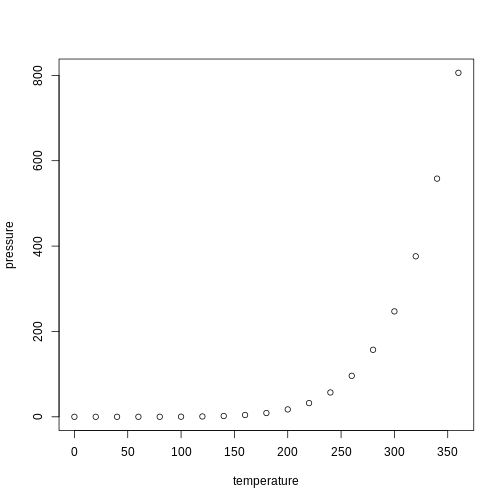
\includegraphics{tesis-rmarkdown_files/figure-latex/pressure-1.pdf}
\caption{Gráfico de presión}
\end{figure}

Tabla con comandos \LaTeX:

\begin{table}[h]
\centering
\begin{tabular}{l*{6}{c}r}
Variable              & Obs 1 & Obs 2 & Obs 3 & Obs 4 & Obs 5\\
\hline
V1 & 6 & 4 & 0 & 2 & 10 \\
V2            & 6 & 3 & 0 & 3 &  8 \\
V3           & 6 & 2 & 1 & 3 &  7 \\
V4     & 6 & 2 & 1 & 3 &  5 \\
\end{tabular}
    \caption{Tabla de ejemplo.}
\end{table}

\hypertarget{refs}{}
\leavevmode\hypertarget{ref-bock2010stats}{}%
Bock, David E, Paul F Velleman, and Richard D De Veaux. 2010.
\emph{Stats: Modeling the World}. Addison-Wesley.

%----------------------------------------------------------------------%


           %%%%%%%%%%%%%%%%%%%%%%%%%%%%%%%%%%%%%%%%%%%%%%%%%%%%
           %   REFERENCIAS 
           %%%%%%%%%%%%%%%%%%%%%%%%%%%%%%%%%%%%%%%%%%%%%%%%%%%%

\cleardoublepage
\nocite{*} % To make all the uncited references to appear in the bibliography.
\bibliographystyle{apacite} 
\bibliography{bibliografia.bib}

%----------------------------------------------------------------------%


%----------------------------------------------------------------------%

           %%%%%%%%%%%%%%%%%%%%%%%%%%%%%%%%%%%%%%%%%%%%%%%%%%%%
           %   INDEX 
           %%%%%%%%%%%%%%%%%%%%%%%%%%%%%%%%%%%%%%%%%%%%%%%%%%%%

%% Uncomment the following lines to include an index.

%% INSERT INDEX PAGE # IN TOC
%%%\addtocounter{chapter}{1}
%%%\addcontentsline{toc}{chapter}{\protect\numberline{\thechapter}{Index}}
%%\addcontentsline{toc}{chapter}{\protect\numberline{}{Index}}
%% NOTE: Insert "\label{IDX}" in '.ind' file after compiling the index
%% with makeindex.
%%\index{ @\label{IDX}}
%% The above NOTE is not really needed as can be achieved by the trick below.
%\addtocounter{page}{1}
%\label{IDX}
%\addtocounter{page}{-1}
%\printindex

%----------------------------------------------------------------------%


\end{document}
%======================================================================%
%%%%%%%%%%%%%%%%%%%%%%%%%%%%%%%%%%%%%%%%%%%%%%%%%%%%%%%%%%%%%%%%%%%%%%%%
%% Local Variables:
%% TeX-command-default: "LaTeX"
%% End:
